\section*{Задание 1. Свободное движение}

Рассмотрим систему 2-го порядка, заданную дифференциальным уравнением
\begin{equation}
    \ddot y +a_1\dot y+a_0y=u.
\end{equation}
Сделаем некоторые преобразования для структурной схемы, которую можно
увидеть в рисунке \ref{fig:task_1_slx} (начальные условия задаются в двух
последних интеграторах):
\begin{equation*}
    \begin{array}{c}
        p^2[y]+p[a_1y]+a_0y=u,\\[2mm]
        y=\frac{1}{p^2}[u-a_0y-a_1\dot y].
    \end{array}
\end{equation*}
Для каждого из вариантов задано по шесть наборов значений корней 
характеристического уравнения $\lambda_1$ , $\lambda_2$ и начальных условия 
$y(0), \dot y(0)$. Чтобы вычислить коэффициенты $a_1$ и $a_0$, 
воспользуемся формулами $a_1=-\lambda_1-\lambda_2$, $a_0=\lambda_1\lambda_2$.
Это все можно увидеть в таблице \ref{tab:values}, а аналитические 
решения свободного движения - уравнения со \ref{eq:11} по \ref{eq:16},
вывод которых можно увидеть в конце документа.
Графики моделирования схемы и сравнения с аналитическими решениями можно
увидеть на рисунке \ref{fig:task_1_out}. Все графики (пары моделирования
и аналитического решения) похожи друг на друга за исключением последнего
шестого набора, в котором колеблется синус (должен быть устойчив по Ляпунову) 
с маленьком амплидой, согласно
аналитическому решению, но моделирование показывает, что система неустойчива,
и у меня нет идей, почему происходит несовпадение. Про остальные наборы: первый,
второй асимптотически устойчивы, третий устойчив по Ляпунову, четвертый
и пятый неустойчивы.


\begin{table}[h!]
    \centering
    \begin{tabular}{|c|c|c|c|c|c|c|c|}
    \hline
    \text{№} & $\lambda_1$ & $\lambda_2$ & $y(0)$ & $\dot{y}(0)$ & $a_0$ & $a_1$ \\
    \hline
    1 & $-3$ & $-1.5$ & $1$ & $0$ & $4.5$ & $4.5$ \\
    \hline
    2 & $-1.2 + j10$ & $-1.2 - j10$ & $1$ & $0$ & $101.44$ & $2.4$ \\
    \hline
    3 & $j10$ & $-j10$ & $1$ & $0$ & $100$ & $0$ \\
    \hline
    4 & $1.2 + j10$ & $1.2 - j10$ & $0.05$ & $0$ & $101.44$ & $-2.4$\\
    \hline
    5 & $3$ & $1.5$ & $0.05$ & $0$ & $4.5$ & $-4.5$\\
    \hline
    6 & $-0.8$ & $0.8$ & $0$ & $0.1$ & $-0.64$ & $0$ \\
    \hline
    \end{tabular}
    \caption{\label{tab:values}Таблица корнями характеристического уравнения, начальными условиями и коэффициентами.}
\end{table}

\begin{equation}
    \label{eq:11}
    y_{\text{св}_1}(t)=2e^{-1.5t}-e^{-3t},
\end{equation}
\begin{equation}
    \label{eq:12}
    y_{\text{св}_2}(t)e^{-1.2t}(\cos 10t-0.12\cdot\sin 10t),
\end{equation}
\begin{equation}
    \label{eq:13}
    y_{\text{св}_3}(t)=\cos10t,
\end{equation}
\begin{equation}
    \label{eq:14}
    y_{\text{св}_4}(t)=e^{1.2t}(0.05\cdot\cos10t-0.006\cdot\sin10t),
\end{equation}
\begin{equation}
    \label{eq:15}
    y_{\text{св}_5}(t)=-0.05e^{3t}+0.1e^{1.5t},
\end{equation}
\begin{equation}
    \label{eq:16}
    y_{\text{св}_6}(t)=0.125\cdot\sin0.8t.
\end{equation}

\begin{figure}
    \centering
    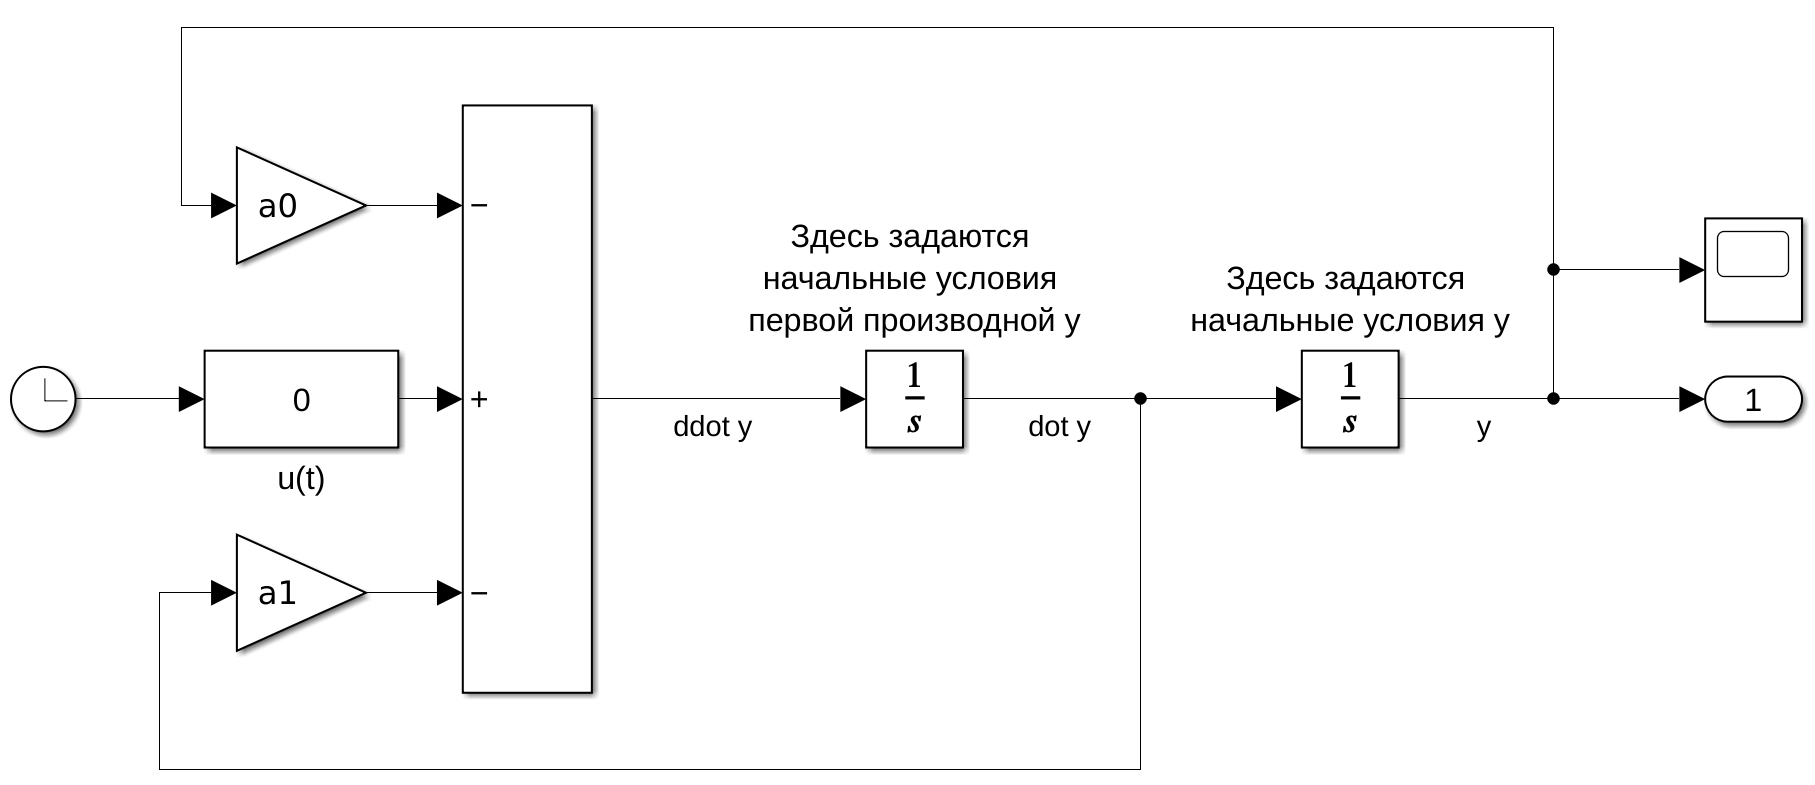
\includegraphics[width=1\textwidth]{figs/task_1_slx.png}
    \caption{Структурная схема дифференциального уравнения задания 1.}
    \label{fig:task_1_slx}
\end{figure}
    
\begin{figure}
    \centering
    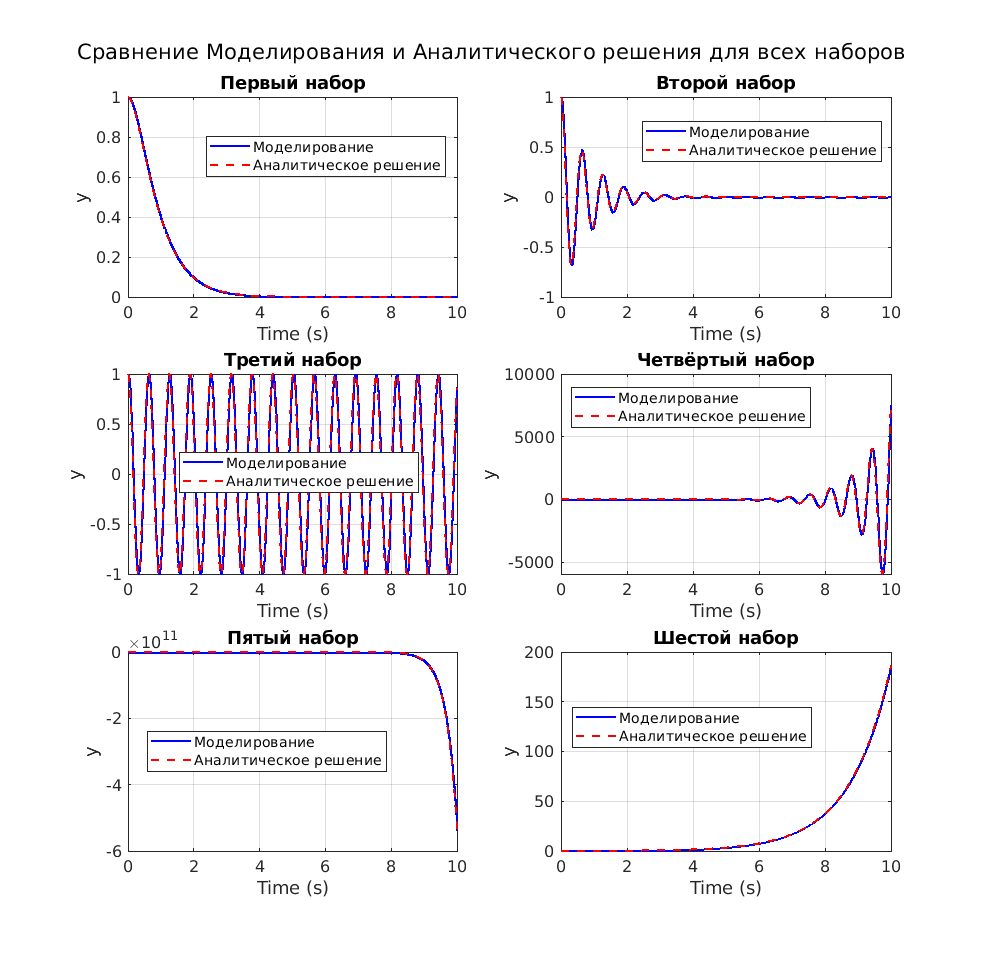
\includegraphics[width=1\textwidth]{figs/task_1_out.png}
    \caption{Графики свободного движения задания 1.}
    \label{fig:task_1_out}
\end{figure}


\section*{Задание 2. Область устойчивости}




\newpage
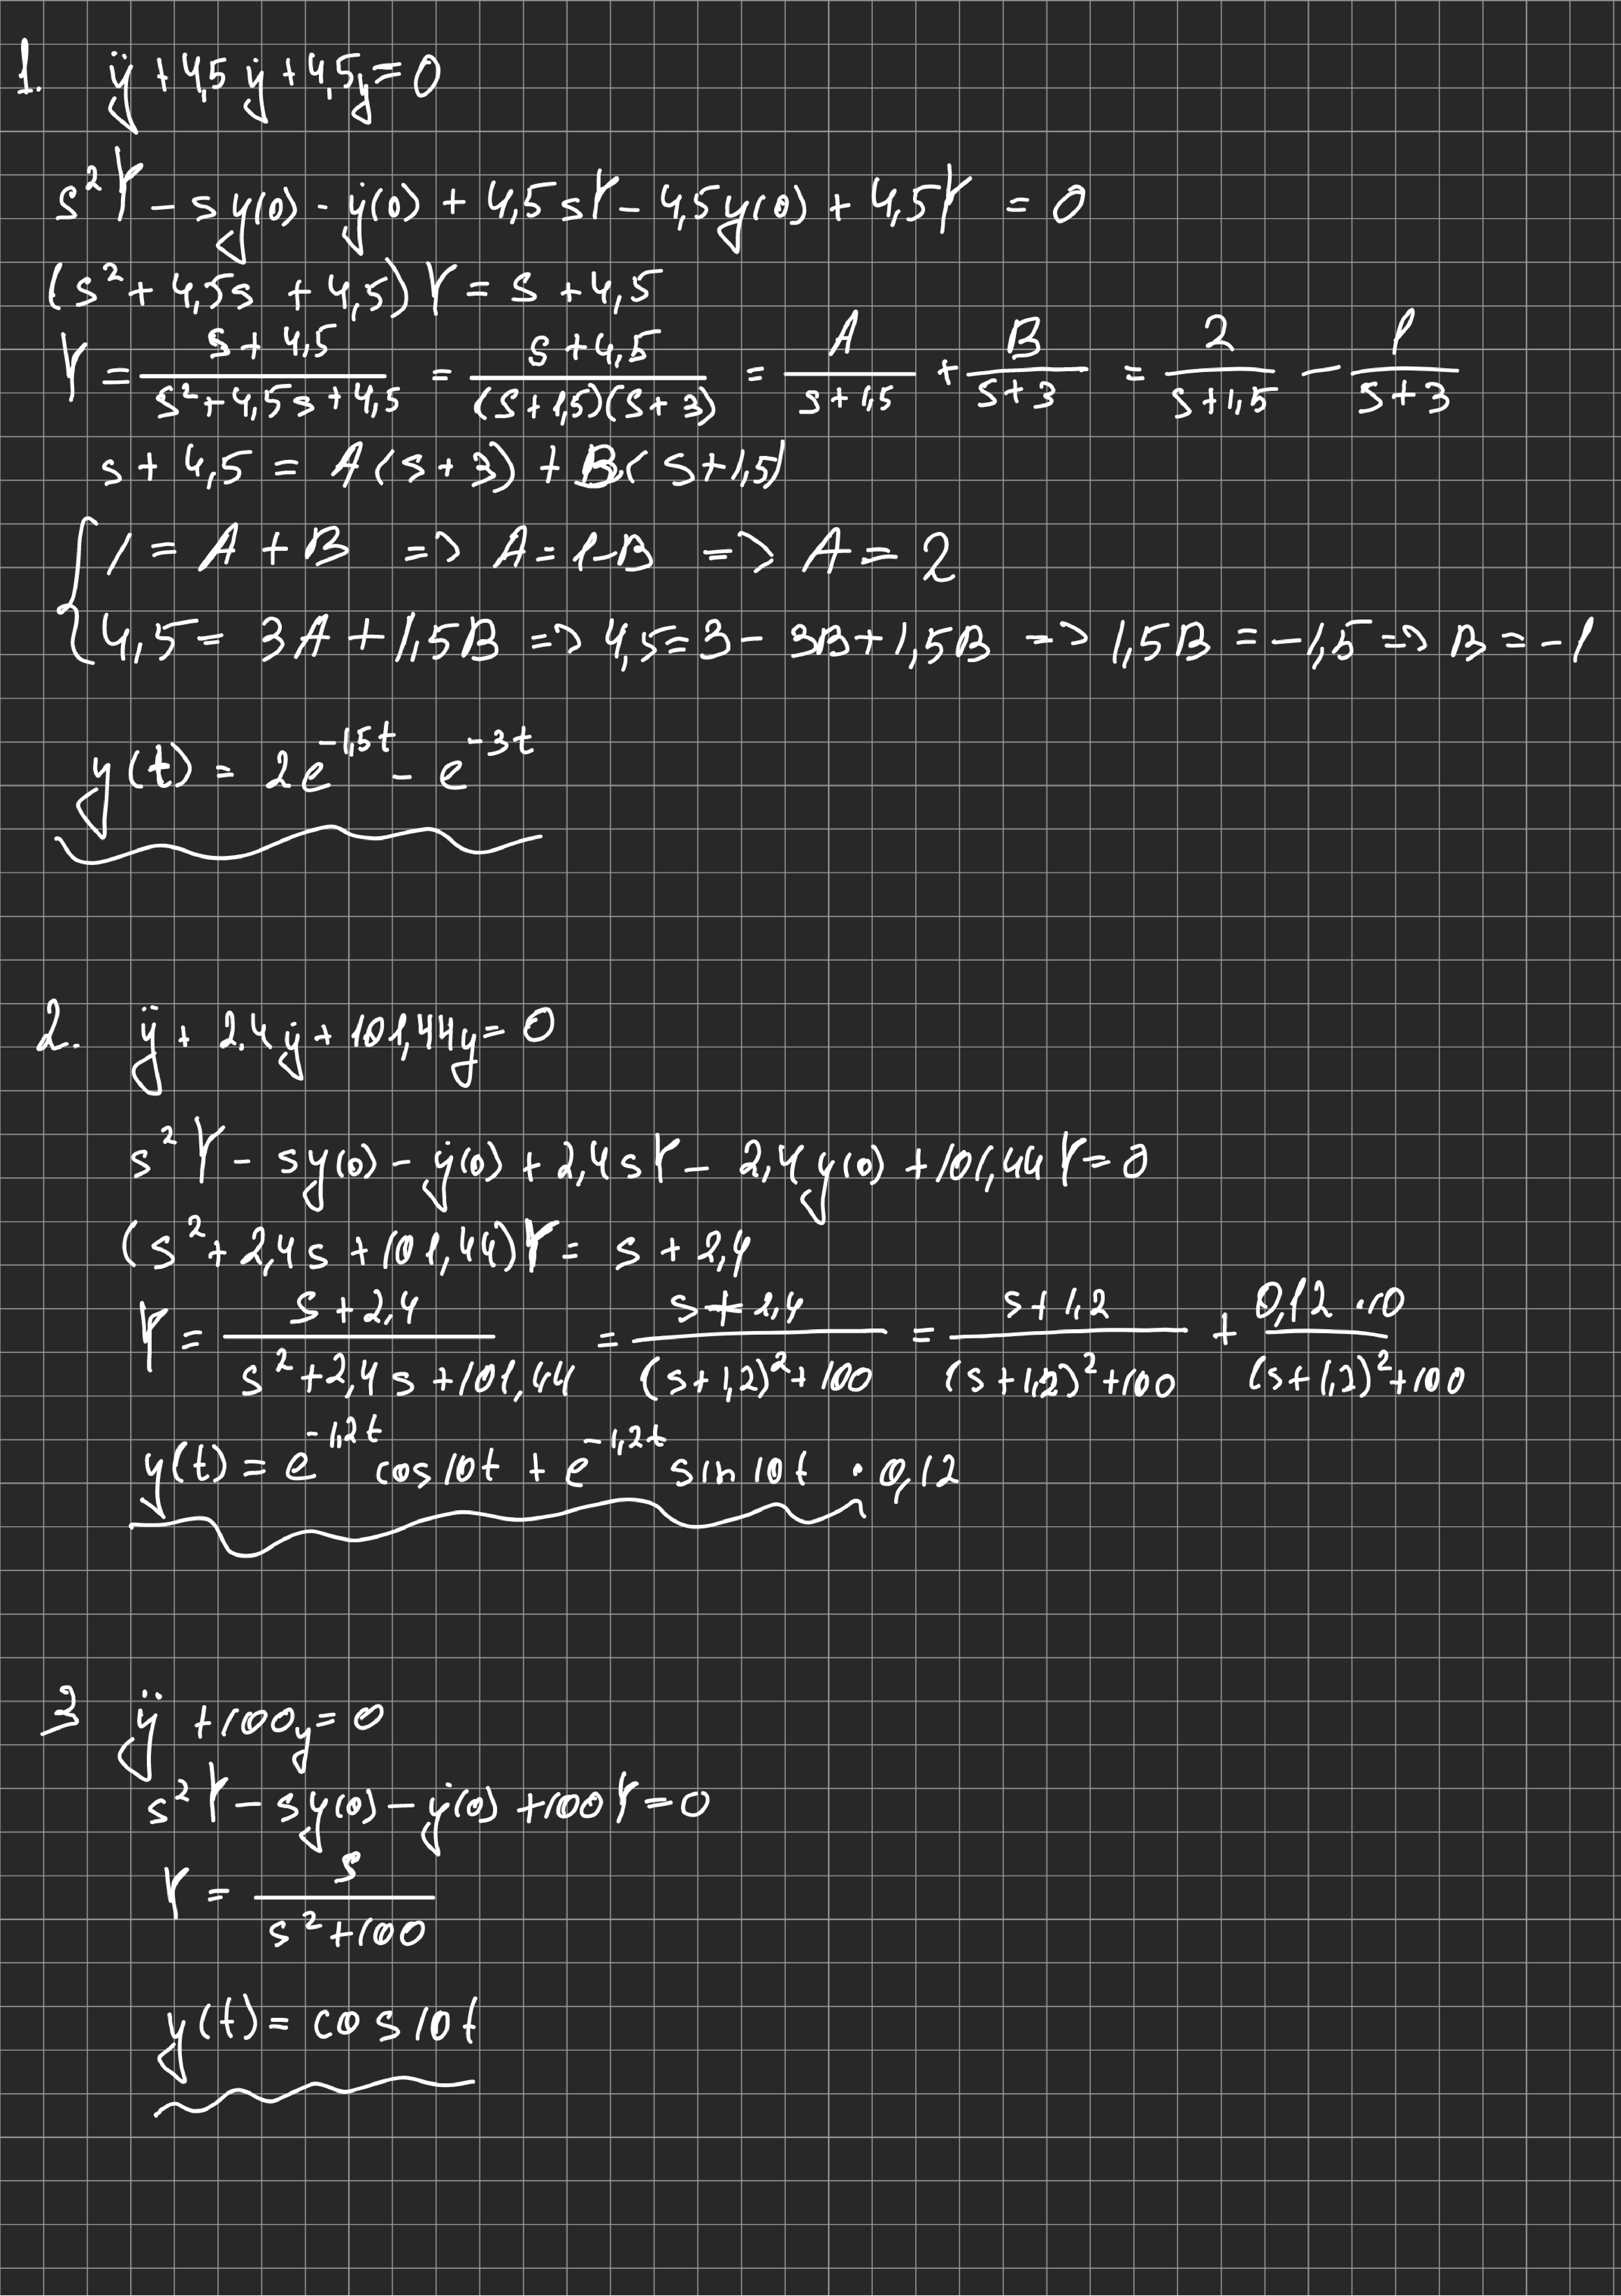
\includepdf[pages=-,scale=1]{figs/analres.pdf}

